
\section{Giá trị lượng giác của một góc lượng giác}
\subsection{Tóm tắt lý thuyết}
\begin{tomtat}
	\subsubsection{Khái niệm góc lượng giác và số đo của góc lượng giác}
	Trong mặt phẳng, cho hai tia $Ou$, $Ov$. Xét tia $Om$ cùng nằm trong mặt phẳng này. Nếu tia $Om$ quay quanh điểm $O$, theo một chiều nhất định từ $Ou$ đến $Ov$, thì ta nói nó quét một góc lượng giác với tia đầu  $Ou$, tia cuối $Ov$ và kí hiệu là ($Ou$, $Ov$).\\
	Mỗi góc lượng giác gốc $O$ được xác định bởi tia đầu $Ou$, tia cuối $Ov$ và số đo của nó.
	\begin{center}
		\begin{minipage}[H]{0.3\textwidth}
			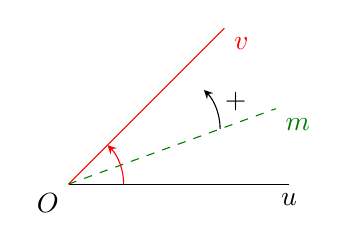
\begin{tikzpicture}[scale=.7]	
				\draw (0,0) -- (4,0)node[below] {$u$};
				\draw[red] (0,0) -- (45:4)node[below right] {$v$};
				\draw[dashed,green!50!black] (0,0) -- (20:4)node[below right] {$m$};
				\draw[-stealth,red] (0:1) arc (0:45:1);
				\draw[-stealth] (2.75,1) arc (0:45:1);
				\path (30:3.5) node[below=-2pt]{$+$};
				\path (0:0) node[below left]{$O$};
			\end{tikzpicture}
		\end{minipage}
		\begin{minipage}[H]{0.3\textwidth}
			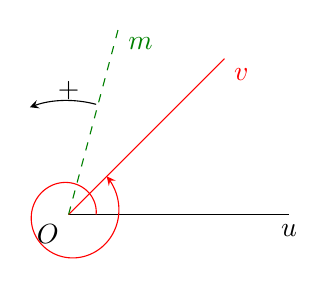
\begin{tikzpicture} [scale=.7]	
				\draw (0,0) -- (4,0)node[below] {$u$};
				\draw[red] (0,0) -- (45:4)node[below right] {$v$};
				\draw[dashed,green!50!black] (0,0) -- (75:3.5)node[below right] {$m$};
				\draw[red,-stealth,smooth,samples=100] plot[domain =0:2.25*pi]({.5*(1.1)^(\x) *cos(\x r)},{.5*(1.1)^(\x) *sin(\x r)});
				\draw[-stealth] (0.5,2) arc (75:110:2);
				\path (90:2.5) node[below=-2pt]{$+$};
				\path (0:0) node[below left]{$O$};
			\end{tikzpicture}
		\end{minipage}
		\begin{minipage}[H]{0.3\textwidth}
			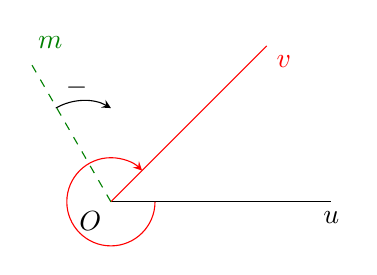
\begin{tikzpicture}[scale=.7]		
				\draw (0,0) -- (4,0)node[below] {$u$};
				\draw[red] (0,0) -- (45:4)node[below right] {$v$};
				\draw[dashed,green!50!black] (0,0) -- (120:3)node[above right] {$m$};
				\draw[-stealth,red] (0:.8) arc (0:-315:.8);
				\draw[-stealth] (-1,1.7) arc (120:60:1);
				\path (105:2.4) node[below=-2pt]{$-$};
				\path (0:0) node[below left]{$O$};
			\end{tikzpicture}
		\end{minipage}
	\end{center}
	\subsubsection{Hệ thức Chasles}
	\immini{Hệ thức Chasles: Với ba tia $Ou$, $Ov$, $Ow$ bất kì, ta có 	
	$$
		\text{sđ}(Ou, Ov)+\text{sđ}(Ov,Ow)=\text{sđ}(Ou,Ow)+k 360^{\circ}(k \in \mathbb{Z}). 
		$$}
	{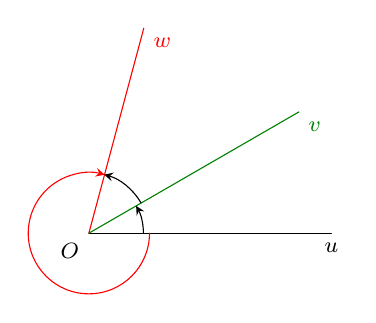
\begin{tikzpicture}[scale=0.77, font=\footnotesize, line join=round, line cap=round, >=stealth]		
			\draw (0,0) -- (4,0)node[below] {$u$};
			\draw[red] (0,0) -- (75:3.5)node[below right] {$w$};
			\draw[green!50!black] (0,0) -- (30:4)node[below right] {$v$};
			\draw[-stealth,red] (0:1) arc (0:-285:1);
			\draw[-stealth] (0:.9) arc (0:30:.9);
			\draw[-stealth] (.86,.5) arc (30:75:1);
			\path (0:0) node[below left]{$O$};
	\end{tikzpicture}}
	% Nhận xét. Từ hệ thức Chasles, ta suy ra:
	% Với ba tia tuỳ ý $Ox$, $Ou$, $Ov$ ta có
	% $$
	% \text{sđ}(Ou, Ov)=\text{sđ}(Ox, Ov)-\text{sđ}(Ox,Ou)+k360^{\circ}(k \in \mathbb{Z}). 
	% $$
	% Hệ thức này đóng vai trò quan trọng trong việc tính toán số đo của góc lượng giác.
	\subsubsection{Đơn vị đo góc và cung tròn}
	\textbf{Đơn vị độ}: Góc $1^{\circ}$ bằng $\dfrac{1}{180}$ góc bẹt.\\
	Đơn vị độ được chia thành những đơn vị nhỏ hơn: $1^{\circ}=60'; 1'=60"$.\\
	% Đối với các góc lượng giác, khi mà số vòng quay trong chuyển động tương ứng từ tia đầu đến tia cuối là khá lớn thì số đo của chúng tính bằng độ sẽ trở nên cồng kềnh. Do đó, trong khoa học và kĩ thuật, bên cạnh việc đo bằng độ, người ta còn sử dụng đơn vị đo góc bằng rađian.\\
	\immini{\textbf{Đơn vị rađian}: Cho đường tròn $(O)$ tâm $O$, bán kính $R$ và một cung $AB$ trên $(O)$.
		Ta nói cung tròn $AB$ có số đo bằng 1 rađian nếu độ dài của nó đúng bằng bán kính $R$.
		Khi đó ta cũng nói rằng góc $AOB$ có số đo bằng 1 rađian và viết: $\overset\frown{AOB}=1$ rad.}
	{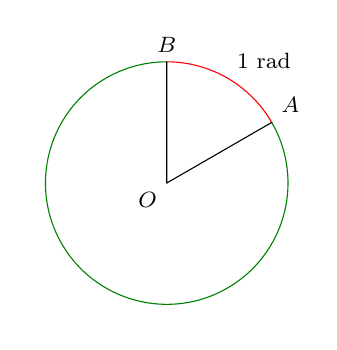
\begin{tikzpicture}[scale=0.77, font=\footnotesize, line join=round, line cap=round, >=stealth]		
			\draw[green!50!black] (30:2) arc (30:-270:2);
			\draw[red] (30:2) arc (30:90:2);
			\draw (90:2)node[above]{$B$}--(0:0)--(30:2)node[above right]{$A$};
			\path (0:0) node[below left]{$O$};
			\draw(60:2) node[above right]{1 rad};
	\end{tikzpicture}}
	\textbf{Quan hệ giữa độ và rađian:}
	$$
	1 \text{ góc bẹt }=180^\circ = 1 \mathrm{rad} \Leftrightarrow  1^\circ=\dfrac{\pi}{180} \mathrm{rad} \quad \text { và }\quad 1\,  \mathrm{rad}=\left(\dfrac{180}{\pi}\right)^\circ.
	$$
	\begin{note}
		Khi viết số đo của một góc theo đơn vị rađian, người ta thường không viết chữ rad sau số đo. Chẳng hạn góc $\dfrac{\pi}{2}$ được hiểu là góc $\dfrac{\pi}{2}$ rad.
	\end{note}
	\begin{note}
		Dưới đây là bảng tương ứng giữa số đo bằng độ và số đo bằng rađian của các góc đặc biệt trong phạm vi từ $0^{\circ}$ đến $180^{\circ}$.
	\end{note}
	\begin{center}
		\renewcommand{\arraystretch}{2}
		\begin{tabular}{|l|c|c|c|c|c|c|c|c|c|}
			\hline Độ & $0^{\circ}$ & $30^{\circ}$ & $45^{\circ}$ & $60^{\circ}$ & $90^{\circ}$ & $120^{\circ}$ & $135^{\circ}$ & $150^{\circ}$ & $180^{\circ}$ \\
			\hline Rađian & 0 & $\dfrac{\pi}{6}$ & $\dfrac{\pi}{4}$ & $\dfrac{\pi}{3}$ & $\dfrac{\pi}{2}$ & $\dfrac{2 \pi}{3}$ & $\dfrac{3 \pi}{4}$ & $\dfrac{5 \pi}{6}$ & $\pi$ \\
			\hline
		\end{tabular}
	\end{center}
	\subsubsection{Độ dài cung tròn}
	Một cung của đường tròn bán kính $R$ và có số đo $\alpha$ rad thì có độ dài $l=R \alpha$.
	\subsubsection{Đường tròn lượng giác}
	\immini{\begin{itemize}
			\item Đường tròn lượng giác là đường tròn có tâm tại gốc toạ độ, bán kính bằng $1$, được định hướng và lấy điểm $A(1 ; 0)$ làm điểm gốc của đường tròn.
			\item Điểm trên đường tròn lượng giác biểu diễn góc lượng giác có số đo $\alpha$ là điểm $M$ trên đường tròn lượng giác sao cho sđ$(OA, OM)=\alpha$.
	\end{itemize}
	\begin{note}
		Góc $\alpha$ và $\beta$ có chung điểm biểu diễn khi \fbox{$\alpha - \beta = k2\pi$} (chẵn lần $\pi$)
		\end{note}}
	{
		\begin{tikzpicture}[line join = round, line cap = round, >=stealth, font=\footnotesize, scale=0.6]
			\tikzset{label style/.style={font=\footnotesize}}
			\path (0,0) coordinate (O)
			(3,0) coordinate (A)
			(0,3) coordinate (B)
			(0,-3) coordinate (B')
			(-3,0) coordinate (A')
			(0:0)++(150:3) coordinate (M)
			($(O)!(M)!(A')$) coordinate (H)
			($(O)!(M)!(B)$) coordinate (K)
			;
			\draw[->] (-4,0) -- (4,0) node[above,blue]{$x$};
			\draw[->] (0,-4) -- (0.,4) node[left,blue]{$y$};
			\draw[orange] (O) circle (3cm);
			\draw[rotate=0,->,green!50!black] (0.5,0) arc (0:150:0.5cm);
			\draw (0.35,0.25) node[above,blue] {$\alpha$};
			\draw[dashed] (H)--(M)--(K);
			\draw[green!50!black] (M)--(O);
			\foreach \p/\r in {A/-45,M/150,H/-90,O/-150,A'/-135,B'/-45,B/45,K/0}
			\fill (\p) circle (1pt) node[shift={(\r:3mm)},blue]{$\p$};
		\end{tikzpicture}
	}
	\subsubsection{Các giá trị lượng giác của góc lượng giác}
	\immini{Gọi $M(x;y)$ là điểm biểu diễn của góc lượng giác $\alpha$ trên đường tròn lượng giác. Khi đó, ta có:
		\begin{itemize}
			\item $\cos\alpha=x.$
			\item $\sin\alpha=y.$
			\item $\tan\alpha=\dfrac{\sin\alpha}{\cos\alpha}=\dfrac{y}{x} ~(x\neq0).$
		\item $\cot\alpha=\dfrac{\cos\alpha}{\sin\alpha}=\dfrac{x}{y} ~(y\neq0).$
	\end{itemize}}
	{\begin{tikzpicture}[line join = round, line cap = round, >=stealth, font=\footnotesize, scale=0.6]
			\tikzset{label style/.style={font=\footnotesize}}
			\path (0,0) coordinate (O)
			(3,0) coordinate (A)
			(0,3) coordinate (B)
			(0,-3) coordinate (B')
			(-3,0) coordinate (A')
			(0:0)++(40:3) coordinate (M)
			($(O)!(M)!(A')$) coordinate (H)
			($(O)!(M)!(B)$) coordinate (K)
			;
			\draw[->] (-4,0) -- (4,0) node[above,blue]{$x$};
			\draw[->] (0,-4) -- (0.,4) node[left,blue]{$y$};
			\draw[orange] (O) circle (3cm);
			\draw[rotate=0,->,green!50!black] (0.7,0) arc (0:40:0.7cm);
			\draw (1,0) node[above,blue] {$\alpha$};
			\draw[dashed] (H)--(M)--(K);
			\draw[green!50!black] (M)--(O);
			\draw[blue,fill=black] (0,2) node[left]{$\sin\alpha$}(2,0) circle(1pt) node[below]{$\cos\alpha$}(3,2.3) node{$M(x;y)$};
			\foreach \p/\r in {A/-45,O/-135,A'/-135,B'/-45,B/45}
			\fill (\p) circle (1pt) node[shift={(\r:3mm)},blue]{$\p$};
	\end{tikzpicture}}
	\begin{note}
		a) Ta còn gọi trục tung là trục sin, trục hoành là trục côsin.\\
		b) Từ định nghĩa ta suy ra:
		\begin{itemize}
			\item $\sin\alpha$, $\cos\alpha$ xác định với mọi giá trị của $\alpha$ và ta có:
			$$-1\leq \sin\alpha\leq 1; \quad -1\leq \cos\alpha\leq 1; \quad \sin(\alpha+k2\pi)=\sin\alpha;\quad \cos(\alpha+k2\pi)=\cos\alpha\,\, (k\in\mathbb{Z}).$$
			\item $\tan\alpha$ xác định khi $\alpha\neq\dfrac{\pi}{2}+k\pi\,\,  (k\in\mathbb{Z})$.
			\item $\cot\alpha$ xác định khi $\alpha\neq k\pi\,\,  (k\in\mathbb{Z})$.
			\item Dấu của các giá trị lượng giác của một góc lượng giác phụ thuộc vào vị trí điểm biểu diễn $M$ trên đường tròn lượng giác.
		\end{itemize}
	\end{note}
	\begin{minipage}[h]{0.6\textwidth}
		\begin{tabular}{c|c|c|c|c|}
			\cline{2-5}
			& \multicolumn{4}{c|}{Góc phần tư} \\ \hline
			\multicolumn{1}{|c|}{Giá trị lượng giác} & I     & II     & III     & IV    \\ \hline
			\multicolumn{1}{|c|}{$\sin \alpha$}     &   $+$    &  $ +$      &    $-$    &   $-$  \\ \hline
			\multicolumn{1}{|c|}{$\cos \alpha$}     &   $+$    &  $ -$      &    $-$    &   $+$  \\ \hline
			\multicolumn{1}{|c|}{$\tan \alpha$}     &   $+$    &  $ -$      &    $+$    &   $-$  \\ \hline
			\multicolumn{1}{|c|}{$\cot \alpha$}     &   $+$    &  $ -$      &    $+$    &   $-$  \\ \hline
		\end{tabular}
	\end{minipage}
	\begin{minipage}[h]{0.6\textwidth}
		\begin{tikzpicture}[line join = round, line cap = round, >=stealth, font=\footnotesize, scale=0.6]
			\tikzset{label style/.style={font=\footnotesize}}
			\path (0,0) coordinate (O)
			(3,0) coordinate (A)
			(0,3) coordinate (B)
			(0,-3) coordinate (B')
			(-3,0) coordinate (A')
			(0:0)++(-60:3) coordinate (M)
			($(O)!(M)!(A')$) coordinate (H)
			($(O)!(M)!(B)$) coordinate (K)
			;
			\draw[->] (-4,0) -- (4,0) node[above,blue]{$x$};
			\draw[->] (0,-4) -- (0.,4) node[left,blue]{$y$};
			\draw[orange] (O) circle (3cm);
			\draw[rotate=0,->,green!50!black] (0.5,0) arc (0:-60:0.5cm);
			\draw (0.75,-0.35) node[blue] {$\alpha$};
			\draw[dashed] (H)--(M)--(K);
			\draw[green!50!black] (M)--(O);
			\draw[blue] (2.5,2.5) node{$I$}(-2.5,2.5) node{$II$}(-2.5,-2.5) node{$III$}(2.5,-2.5) node{$IV$};
			\foreach \p/\r in {A/-45,M/-60,H/90,O/-150,A'/-135,B'/-45,B/45,K/180}
			\fill (\p) circle (1pt) node[shift={(\r:3mm)},blue]{$\p$};
		\end{tikzpicture}
	\end{minipage}
	% \subsubsection{Giá trị lượng giác của các góc đặc biệt}
	% \begin{center}
	% 	\renewcommand{\arraystretch}{2}
	% 	\begin{tabular}{|c|c|c|c|c|c|}
	% 		\hline
	% 		\multirow{2}{*}{Góc $\alpha$} & $0$              & $\dfrac{\pi}{6}$  & $\dfrac{\pi}{4}$  & $\dfrac{\pi}{3}$  & $\dfrac{\pi}{2}$              \\ \cline{2-6} 
	% 		& $0^\circ$              & $30^\circ$  & $45^\circ$  & $60^\circ$  & $90^\circ$             \\ \hline
	% 		$\sin\alpha$                  & $0$             & $\dfrac{1}{2}$ & $\dfrac{\sqrt{2}}{2}$ & $\dfrac{\sqrt{3}}{2}$ & 1              \\ \hline
	% 		$\cos\alpha$                  & $1$             & $\dfrac{\sqrt{3}}{2}$ & $\dfrac{\sqrt{2}}{2}$ & $\dfrac{1}{2}$ & 0              \\ \hline
	% 		$\tan\alpha$                 & $0$             & $\dfrac{1}{\sqrt{3}}$ & 1 & $\sqrt{3}$ & Không xác định \\ \hline
	% 		$\cot\alpha$                  & Không xác định & $\sqrt{3}$ & 1 & $\dfrac{1}{\sqrt{3}}$ & 0              \\ \hline
	% 	\end{tabular}
	% \end{center}
	\subsubsection{Các công thức lượng giác cơ bản}
	Đối với các giá trị lượng giác, ta có các hệ thức cơ bản sau
	\begin{enumEX}[$\bullet$]{2}
		\item $\sin^2 \alpha  + \cos^2 \alpha =1$
		\item $ 1+ \tan^2 \alpha= \dfrac{1}{\cos^2 \alpha}$ $\left(\alpha \neq \dfrac{\pi}{2}+k\pi , k\in \mathbb{Z}\right)$
		\item $ 1+ \cot^2 \alpha= \dfrac{1}{\sin^2 \alpha}$ $\left(\alpha \neq k\pi , k\in \mathbb{Z}\right)$
		\item $\tan \alpha \cdot \cot \alpha =1 $ $\left(\alpha \neq \dfrac{k\pi}{2}, k\in \mathbb{Z}\right)$
	\end{enumEX}
	\newpage
	\subsubsection{Giá trị lượng giác của các góc có liên quan đặc biệt}
	\begin{enumerate}
		\item Góc đối nhau ($\alpha$ và $-\alpha$)
		\immini{\begin{itemize}
				\item $\cos (-\alpha)=\cos \alpha$
				\item $\sin (-\alpha) =-\sin \alpha$
				\item $\tan (-\alpha) =-\tan \alpha$
				\item $\cot (-\alpha) =-\cot \alpha$
		\end{itemize}}
		{\vspace*{-1cm}\begin{tikzpicture}[line join = round, line cap = round, >=stealth, font=\footnotesize, scale=0.5]
				\tikzset{label style/.style={font=\footnotesize}}
				\path (0,0) coordinate (O)
				(3,0) coordinate (A)
				(0:0)++(120:3) coordinate (M)
				(0:0)++(-120:3) coordinate (N)
				(0,4) coordinate (C)
				(0,-4) coordinate (D)
				($(O)!(M)!(C)$) coordinate (E)
				($(O)!(N)!(D)$) coordinate (F)
				;
				\draw[->] (-4,0) -- (4,0) node[above,blue]{$x$};
				\draw[->] (0,-4) -- (0.,4) node[left,blue]{$y$};
				\draw[orange] (O) circle (3cm);
				\draw[rotate=0,->,red] (0.5,0) arc (0:120:0.5cm);
				\draw[rotate=0,->,green!50!black] (0.6,0) arc (0:-120:0.6cm);
				\draw (0,0) node[above right=2pt,blue] {$\alpha$} (0,-0) node[below right=2pt,blue]{$-\alpha$};
				\draw[dashed] (E)--(M)--(N)--(F);
				\draw[green!50!black] (M)--(O);
				\draw[red] (N)--(O);
				\foreach \p/\r in {A/-45,M/120,N/-120,O/-150}
				\fill (\p) circle (1pt) node[shift={(\r:3mm)},blue]{$\p$};
		\end{tikzpicture}}
		\item Góc bù nhau ($\alpha$ và $\pi-\alpha$)
		\immini{\begin{itemize}
				\item $\sin (\pi -\alpha)=\sin \alpha$
				\item $\cos (\pi -\alpha) =-\cos \alpha$
				\item $\tan (\pi -\alpha) =-\tan \alpha$
				\item $\cot (\pi -\alpha) =-\cot \alpha$
		\end{itemize}}
		{\vspace*{-0.5cm}\begin{tikzpicture}[line join = round, line cap = round, >=stealth, font=\footnotesize, scale=0.5]
				\tikzset{label style/.style={font=\footnotesize}}
				\path (0,0) coordinate (O)
				(3,0) coordinate (A)
				(0:0)++(30:3) coordinate (M)
				(0:0)++(150:3) coordinate (N)
				(4,0) coordinate (C)
				(-4,0) coordinate (D)
				($(O)!(M)!(C)$) coordinate (E)
				($(O)!(N)!(D)$) coordinate (F)
				;
				\draw[->] (-4,0) -- (4,0) node[above,blue]{$x$};
				\draw[->] (0,-4) -- (0.,4) node[left,blue]{$y$};
				\draw[orange] (O) circle (3cm);
				\draw[rotate=0,->,red] (0.5,0) arc (0:150:0.5cm);
				\draw[rotate=0,->,green!50!black] (1.6,0) arc (0:30:1.6cm);
				\draw (2,0) node[above,blue] {$\alpha$} (0.3,1.5) node[below,blue]{$\pi-\alpha$};
				\draw[dashed] (E)--(M)--(N)--(F);
				\draw[red] (O)--(N);
				\draw[green!50!black] (O)--(M);
				\foreach \p/\r in {A/-45,M/30,N/150,O/-130}
				\fill (\p) circle (1pt) node[shift={(\r:3mm)},blue]{$\p$};
		\end{tikzpicture}}
		\item Góc phụ nhau ($\alpha$ và $\dfrac{\pi}{2}-\alpha$)
		\immini{\begin{itemize}
				\item $\sin \left( \dfrac{\pi}{2}-\alpha\right)=\cos \alpha$
				\item $\cos \left( \dfrac{\pi}{2}-\alpha\right)=\sin \alpha$
				\item $\tan \left( \dfrac{\pi}{2}-\alpha\right)=\cot \alpha$
				\item $\cot \left( \dfrac{\pi}{2}-\alpha\right)=\tan \alpha$
		\end{itemize}}
		{\vspace*{-0.5cm}\begin{tikzpicture}[line join = round, line cap = round, >=stealth, font=\footnotesize, scale=0.5]
				\tikzset{label style/.style={font=\footnotesize}}
				\path (0,0) coordinate (O)
				(3,0) coordinate (A)
				(0:0)++(20:3) coordinate (M)
				(0:0)++(70:3) coordinate (N)
				(0,4) coordinate (C)
				(4,0) coordinate (D)
				($(O)!(M)!(C)$) coordinate (E)
				($(O)!(N)!(D)$) coordinate (F)
				(2.82,0) coordinate (G)
				(0,2.82) coordinate (H)
				;
				\draw[->] (-4,0) -- (4,0) node[above,blue]{$x$};
				\draw[->] (0,-4) -- (0.,4) node[left,blue]{$y$};
				\draw[orange] (O) circle (3cm);
				\draw[rotate=0,->,red] (0.7,0) arc (0:70:0.7cm);
				\draw[rotate=0,->,green!50!black] (1.6,0) arc (0:20:1.6cm);
				\draw (2,0) node[above,blue] {$\alpha$} (1,-.2) node[below,blue]{$\frac{\pi}{2}-\alpha$};
				\draw[dashed] (E)--(M) (F)--(N) (G)--(M) (H)--(N);
				\draw[dashed] (-3,-3)--(3,3);
				\draw[->] (0.8,-.5)--(0.5,0.45);
				\draw[red] (O)--(N);
				\draw[green!50!black] (O)--(M);
				\foreach \p/\r in {A/-45,M/20,N/70,O/-220}
				\fill (\p) circle (1pt) node[shift={(\r:3mm)},blue]{$\p$};
		\end{tikzpicture}}
		\item Góc hơn kém $\pi$ ($\alpha$ và $\pi+\alpha$)
		\immini{\begin{itemize}
				\item $\sin (\pi +\alpha)=-\sin \alpha$
				\item $\cos (\pi +\alpha)=-\cos \alpha$
				\item $\tan (\pi +\alpha)=\tan \alpha$
				\item $\cot (\pi +\alpha)=\cot \alpha$
		\end{itemize}}
		{\vspace*{-0.5cm}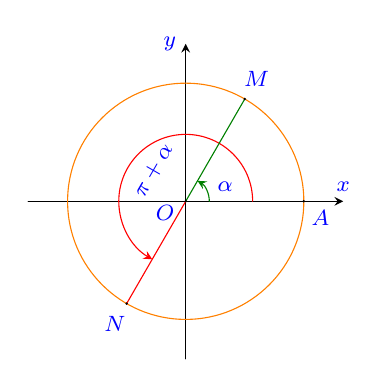
\begin{tikzpicture}[line join = round, line cap = round, >=stealth, font=\footnotesize, scale=0.5]
				\tikzset{label style/.style={font=\footnotesize}}
				\path (0,0) coordinate (O)
				(3,0) coordinate (A)
				(0:0)++(60:3) coordinate (M)
				(0:0)++(240:3) coordinate (N)
				;
				\draw[->] (-4,0) -- (4,0) node[above,blue]{$x$};
				\draw[->] (0,-4) -- (0.,4) node[left,blue]{$y$};
				\draw[orange] (O) circle (3cm);
				\draw[rotate=0,->,red] (1.7,0) arc (0:240:1.7cm);
				\draw[rotate=0,->,green!50!black] (0.6,0) arc (0:60:0.6cm);
				\draw (1,0) node[above,blue] {$\alpha$};
				\draw (-1.2,1) node[below,blue,rotate=60]{$\pi+\alpha$};
				\draw[red] (O)--(N);
				\draw[green!50!black] (O)--(M);
				\foreach \p/\r in {A/-45,M/60,N/240,O/-150}
				\fill (\p) circle (1pt) node[shift={(\r:3mm)},blue]{$\p$};
		\end{tikzpicture}}
	\end{enumerate}
\end{tomtat}
